\chapter{Stand der Technik}

In diesem Kapitel werden die aktuelle technische Lösungen im Bereich Cloud Computing und verteiltes Rechnen vorgestellt, sowie die gängigsten Softwarewerkzeuge mit denen diese Systeme erzeugt und verwaltet werden können.

\section{Cloud Computing}
Cloud Computing besitzt in der Literatur mehrere Definitionen.\cite{Marston2011} Die am weitesten verbreitete Definition wurde vom National Institute of Standards and Technology (NIST) festgelegt.Nach dieser Definition ist Cloud Computing ein Modell, das einen allgegenwärtigen, bequemen, bedarfsgerechten Zugang zu einem gemeinsamen Pool an konfigurierbarer Rechenressourcen die jederzeit und von jedem Ort aus über das Internet oder ein Netzwerk schnell zur Verfügung gestellt 
werden können. Es wird durch fünf Eigenschaften charakterisiert:   \\
\begin{itemize}
	\item On-Demand und Selbstbedienung: Kunden können die Rechenressourcen selbständig nach Bedarf ohne menschliche Interaktion anfordern
	\item Breiter Netzzugang: Ressourcen sind über Netzwerkverbindung erreichbar über standardisierte Zugriffsmechanismen
	\item Ressourcen-Pooling: Die Ressourcen des Anbieters werden aus mehreren physikalischen Recheneinheiten zusammengelegt, die auch geographisch nicht an einem Ort sein müssen. Mit einem Multi-Tenant Modell werden die Ressourcen dynamisch je nach Kundenbedarf zugewiesen. Der Kunde hat keinen Kenntnis oder Kontrolle über den genauen Standort der bereitgestellten Ressourcen.
	\item Schnelle Elastizität: Bereitgestellte Ressourcen können flexibel bereitgestellt und freigegeben werden. Für den Kunden erscheint die Menge der bereitgestellten Ressourcen unbegrenzt, sie können jederzeit in beliebiger Menge gebucht werden.
	\item Measured Service: Nutzung der Cloud Systeme wird automatisch gemessen und optimiert anhand einer Messfunktion, die nach Metriken wie Speicher, Verarbeitung, Bandbreite und Benutzerknoten die Ressourcennutzung ermittelt. Kosten für den Cloud Dienst werden nach der gemessenen Nutzung ermittelt (Pay per use) \cite{Mell2011}
\end{itemize}

Cloud Computing ist ein Geschäftsmodell für die Bereitstellung von IT Infrastruktur, Komponenten und Anwendungen, welches mittlerweile den Markt dominiert. \cite{Benlian2018} Cloud Service Anbieter betreiben die IT Infrastruktur und stellen sie für Kunden zur Verfügung. Kunden müssen nicht ihre eigene Infrastruktur aufbauen, sie können die benötigten Kapazitäten je nach aktueller Bedarf einkaufen. Diese Lösung ermöglicht den Kunden hohe Rechenkapazitäten zu erhalten, die diese selber nicht aufbauen und betreiben können.\cite{Arasaratnam2011} Der Markt für Cloud Infrastruktur ist ein weiterhin wachsender Markt (Stand Q4 2023) mit 270 Milliarden US Dollar Gesamtausgaben für das Jahr 2023. Die größten Cloud Service Anbieter und deren Marktanteil ist in der Tabelle \ref{cloud_marktanteile} aufgelistet.

\begin{table}
	\centering
		\caption{Cloud Anbieter und deren Marktanteile in Q4 2023}
		\label{cloud_marktanteile}
		\begin{tabular}{|c | c|} 
			\hline
			Anbieter & Marktanteil in Prozent \\
			\hline\hline
			AWS & 31\%\\ 
			\hline
			Azure & 24\% \\
			\hline
			Google Cloud & 11\% \\
			\hline
			Alibaba Cloud & 4\% \\
			\hline
			salesforce & 3\% \\
			\hline
			IBM Cloud & 2\% \\ 
			\hline
			ORACLE & 2\% \\ 
			\hline
			Tencent Cloud & 2\% \\ 
			\hline
		\end{tabular}
\end{table}

In der heutigen Zeit sind viele im Alltag verbreitete Applikationen als Cloud Service ausgelegt. Datenspeicherung (Dropbox, Google Drive), Dokumente bearbeiten (Office 365, Google Docs), Business-management (SAP ByDesign) und Videospiele (Geforce Now) sind typische Anwendungsbereiche hierfür. Cloud Computing kann verschiedene Geschäftsmodelle für Kunden anbieten, die je nach Kundenbedarf fertigen Softwareplattform oder reine Rechenressourcen für eigene Applikationen bereitstellen:

\begin{itemize}
	\item Software as a Service (SaaS): Cloud Anbieter stellt den Kunden eine oder mehrere vom Cloud Anbieter angebotene Applikationen zur Verfügung. Der Anbieter übernimmt die Einrichtung von Laufzeitumgebung und Bereitstellung der benötigten Rechenressourcen. Kunde Kann die Software durch bereitgestellten Software Interface über Netzwerk/Internet benutzen und konfigurieren. 
	\item Platform as a Service (PaaS): Kunde lässt eine eigene Applikation auf der Cloud Infrastruktur ausführen. Cloud Anbieter übernimmt die Einrichtung der Laufzeitumgebung fü die Applikation, sowie die Zuteilung der benötigten Rechenressourcen. 
	\item Infrastructure as a Service (IaaS): Kunde kauft Rechenressourcen nach Bedarf ein, Cloud Anbieter stellt eine \gls{virtuelle Maschine} dem Kunden zur Verfügung. Kunde muss die Laufzeitumgebung und Software selber einrichten und betreiben. 
\end{itemize} \cite{Mell2011}

\section{Distributed Computing}

Distributed Computing bezeichnet verteilte Systeme, die aus dem Zusammenschluss von mehreren physikalischen Recheneinheiten bestehen. Auf dieser Weise können sie an einem gemeinsamen Problem arbeiten. Hierdurch ist es möglich auch große Datenmengen oder komplexe Rechenaufgaben effizienter zu verarbeiten als mit einzelnen Recheneinheiten. \cite{AWS2023} Die einzelnen Recheneinheiten in einem Verteilten System werden als Nodes genannt. \cite{ord1994scale} Verteilte Systeme sind heutzutage Stand der Technik, da die Rechenleistung von einzelnen Rechenkernen nicht beliebig skalierbar ist. Wenn also hohe Rechenleistung benötigt wird, kann dies  durch die Zusammenschaltung von mehreren Recheneinheiten und die Parallelisierung von Rechenaufgaben erfolgen, die den Ansatz der Distributed Computing verfolgt. Verteiltes Rechnen bildet die Grundlage für Cloud Computing, da die dafür benötigten Ressourcen mit einzelnen physikalischen Rechnern nicht realisierbar sind. Heutzutage verbreitete Cloud Dienste Provider (Google, Facebook) verwenden verteilte Systeme für ihre Infrastruktur. \cite{arpaci2018operating} 

\section{Edge Computing}

Edge Computing ist eine Form von Distributed Computing. In diesem Kontext werden die Endgeräte, wo Daten entstehen oder benötigt werden als Edge bezeichnet. Durch die zunehmende Digitalisierung der Stadt Infrastruktur und alltägliche Gegenstände wie Mobiltelefone, Uhren, Hausgegenstände entstehen immer höhere Datenmengen, die verarbeitet werden müssen. Im Cloud Computing Ansatz werden die Daten in geographisch weit entfernten Cloud Servern verarbeitet und wieder an die Endgeräte auf der Edge Ebene zurückgesendet. Hierdurch erhöht sich die Latenz sowie die insgesamt benötigte Netzwerkbandbreite. Edge Computing verlagert die Datenverarbeitung in die Nähe der Geräte, wo die Daten entstehen und die verarbeiteten Daten benötigt werden, also in die Edge Ebene und reduziert damit die Latenz und die benötigte Gesamtbandbreite zu entfernten Cloud Servern. \cite{Wang2019} Motiviert wird diese Entwicklung dadurch, dass Netzwerkbandbreite sich deutlich langsamer entwickelt als die Zunahme an erzeuge Datenmengen.\cite{Shi2016} Latenzreduzierung ist relevant für Echtzeitsysteme wie Datenauswertung für autonome Fahrzeuge, aber auch für Anwendungen, wo Berührungsrückmeldungen an dem Benutzer zurückgemeldet werden sollen. Damit der Mensch keinen Latenz empfindet, muss die Kommunikation und Datenverarbeitung innerhalb von 1 ms erfolgen. \cite{Varsha2017} Edge Computing ist eine Alternative für lokale Berechnungen auf dem jeweiligen Endgerät. Diese Endgeräte haben in vielen Fällen nur begrenzte Rechenleistung, so dass die lokale Datenverarbeitung nicht sinnvoll umsetzbar ist. Rechenoperationen können auch in Cloud Systeme ausgelagert werden, allerdings resultiert dieser Ansatz in höhere Latenzen und Bandbreitenauslastungen. \cite{Lin2020} 

\section{Applikationsmanagement in Cloud Systemen}

Applikationen haben in den meisten Fällen Abhängigkeiten zu weiteren Softwarekomponenten, die auf dem ausführenden Betriebssystem installiert werden muss. Das Betriebssystem und die darauf installierte Softwarekomponenten nennt man Laufzeitumgebung. Verschiedene Applikationen können verschiedene Versionen von zusätzlichen Softwarekomponenten nutzen, so dass sie nicht gleichzeitig auf dem selben Betriebssystem und Laufzeitumgebung ausführbar sind. In traditionellen Architekturen wird deswegen eine begrenzte Anzahl an Applikationen mit kompatibler Laufzeitumgebung auf einer physikalischen Maschine ausgeführt, die in eine nicht optimale Auslastung der Hardwareressourcen resultiert. Um die Auslastung zu optimieren, wurde das Konzept der Virtualisierung entwickelt. Die physische Ressourcen werden in mehrere virtuelle Ressourcen aufgeteilt. Hierdurch ist es möglich auf einer physikalischen Maschine mehrere voneinander unabhängige Laufzeitumgebungen einzurichten. Virtualisierung wurde bereits in den 1960-er Jahren entwickelt, allerdings wurde dafür spezielle Hardware benötigt. Für die aktuell verbreitete x86-er Architektur wurde die Virtualisierung von VMWare in 1999 umgesetzt. \cite{Bugnion2012} In der Informationstechnik haben sich zwei Virtualisierungsmethoden durchgesetzt, die in den folgenden Abschnitten vorgestellt werden. Ein Überblick über die Struktur der beiden Methoden im Vergleich zu einem klassischen System ohne Virtualisierung ist in der Abbildung \ref{virtualisierung_optionen} dargestellt. 

\begin{figure}
	\centering
	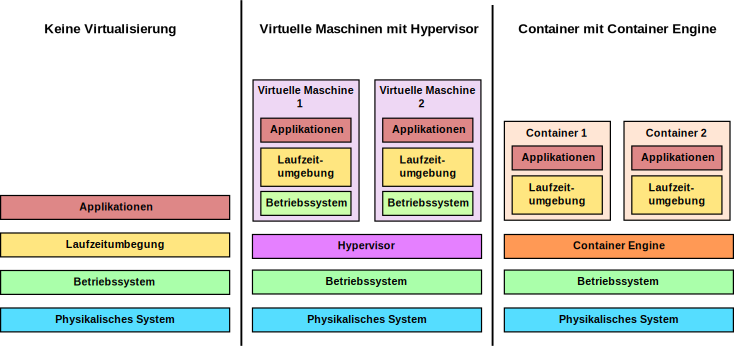
\includegraphics[width=\textwidth]{./content/graphics/applikation_management.pdf}
	\caption{Vergleich keine Virtualisierung zu den beiden verwendeten Virtualisierungsansätzen}
	\label{virtualisierung_optionen}
\end{figure}

\subsection{Virtuelle Maschine}

In Cloud Systemen wurden in den letzten Jahrzehnten hauptsächlich virtuelle Maschinen als Virtualisierungsumgebung verwendet. Bei dieser Methode wird ein neues virtuelles System mit eigenem Betriebssystem erzeugt. Diese neue Umgebungen werden Virtuelle Maschinen bezeichnet. \cite{Pahl2015}  Auf einem Physikalischen System können mehrere virtuelle Maschinen gleichzeitig ausgeführt werden. Virtualisierungssoftware, die für den Einsatz auf Servern entwickelt wurden, nutzen einen sogenannten Hypervisor, um die Virtuelle Maschinen auf dem Server verwalten zu können. Diese Hypervisor können entsprechend virtuelle Maschinen erstellen, löschen, starten und stoppen und ermöglichen damit eine automatisierte Verwaltung. Dieser Ansatz ermöglicht auch die Verwendung von verschiedenen Betriebssystemen in verschiedene virtuelle Maschinen die auf dem selben physikalischen System laufen und bietet damit eine hohe Flexibilität bei den bereitgestellten Laufzeitumgebung für die jeweiligen Applikationen die in der Umgebung ausgeführt werden. Die schematische Darstellung eines Systems mit mehreren virtuellen Maschinen ist in der Abbildung \ref{virtualisierung_optionen} in der mittleren Spalte dargestellt. Applikationen in virtuelle Maschinen auszuführen hat gegenüber keine Virtualisierung auch Nachteile. Hauptnachteil der virtuellen Maschinen ist die zusätzliche Ressourcenaufwand. Für jede unterschiedliche Instanz einer virtuellen Maschine muss ein zusätzliches Betriebssystem mit entsprechenden Laufzeitumgebung zusätzlich zu der auszuführenden Applikation vorhanden sein. Hierdurch ergibt sich eine deutlich höhere Festplattenspeicher und Arbeitsspeicher Auslastung. Ebenfalls wird für das Ausführen des Betriebssystems in der virtuellen Maschine zusätzliche Rechenleistung benötigt. \cite{Mavridis2019} 

\subsection{Container}

Um die vorhin genannte Nachteile der virtuellen Maschinen zu umgehen, haben sich Container als alternative Methode für Virtualisierung in den letzten Jahren verbreitet. Containerisierung ist eine Virtualisierungsmethode, die im Gegensatz zu virtuellen Maschinen keine neue Betriebssysteme für neue virtuelle Umgebungen ausführt. Applikationen werden direkt auf dem Betriebssystem des physikalischen Systems ausgeführt.  Hierdurch sind Container kleiner, da sie kein Betriebssystem zusätzlich enthalten müssen im Vergleich zu virtuelle Maschinen. Container sind durch das Wegfallen des zusätzlichen Betriebssystems auch effizienter im Bezug auf Rechenressourcen. Zusätzlich können Container auch deutlich schneller gestartet werden da kein Betriebssystem beim Startvorgang gebootet werden muss (etwa 50ms bei Container, 30-40s bei virtuelle Maschinen). \cite{Martin2018} Ähnlich wie virtuelle Maschinen auf einem System durch den Hypervisor verwaltet werden können, werden Container mit einem Container Runtime Softwaremodul verwaltet. Die systematische Darstellung eines Systems mit Container als Virtualisierungsmethode ist in der Abbildung \ref{virtualisierung_optionen} in der rechten Spalte dargestellt. 

